\chapter{Géométrie dans $\mathbb{R}^2$ et $\mathbb{R}^3$}

\section{Géométrie dans $\mathbb{R}^2$}

Équation de droite : 
\[\begin{array}{rclr}
x &=& constante &\text{(droite vertical)}\\
y &=& constante & \text{(droite horizontal)} \\
y &=& ax+b, (a, b) \in \mathbb{R}^2 & \text{(toutes les droites non verticales)}
\end{array}\]

En général, l'équation $ax + by + c = 0 (E)$ est l'équation d'une droite $D$. Avec $a \neq 0$ ou $b \neq 0$

\[D = \{(x, y) \in \mathbb{R}^2 | ax + by + c = 0 \}\]

\subsection{Pente et vecteur directeur}

\begin{wrapfigure}[6]{r}{0pt}
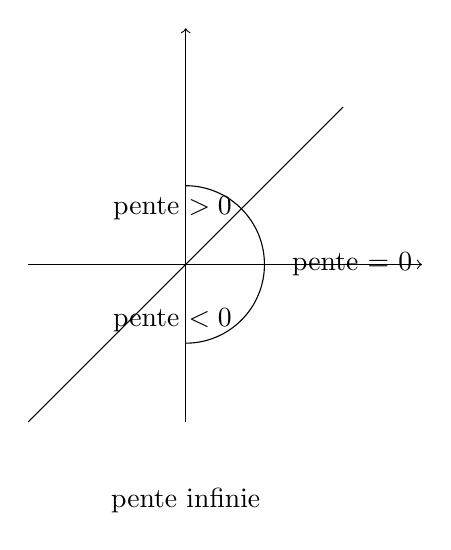
\begin{tikzpicture}
	\draw[->] (-2, 0) -- (3, 0);
	\draw[->] (0, -2) -- (0, 3);

	\draw[] (-2, -2) -- (2, 2);
	\node[left] at (3, 0) {pente = 0};
	\draw[] (1, 0) arc (0:90:1) node [midway, left] {pente $> 0$};
	\draw[] (1, 0) arc (0:-90:1) node [midway, left] {pente $< 0$};
	\node at (0, -3) {pente infinie};
\end{tikzpicture}
\end{wrapfigure}

D d'équation $y =ax + b$ a pour pente a

D d'équation $ax + by + c = 0$
\begin{itemize}
	\item $b \neq 0, (E) \Leftrightarrow y = -\frac{a}{b}x - \frac{c}{b}$. La pente est $-\frac{a}{b}$
	\item $b=0$ a pour pente infini.
\end{itemize}

Une droite D et ses paralléles correspondent à une pente
\begin{itemize}
	\item correspondent à une pente
	\item correspondent un vecteur directeur (et ses multiples)
\end{itemize}

Un vecteur directeur est un vecteur qui "porte" la droite D

\[\vec{u} = \begin{pmatrix}
	u_1 \\
	u_2
\end{pmatrix} = \overrightarrow{OU} \text{ où } U = (u_1, u_2)\]

D d'équation $ax +by +c = 0$.
Un vecteur directeur est donné :
\[\vec{v} = \begin{pmatrix}
	1 \\
	p
\end{pmatrix} \text{ avec } \text{ la pente si } p \in \mathbb{R}\]

\[\vec{v} = \begin{pmatrix}
	0 \\
	1
\end{pmatrix} \text{ si } p \text{ est infinie }\]

\paragraph{Remarque} On se donne 2 points sur D, $A = (x_A, y_A), B=(x_B, y_B)$ 
\[\vec{v} = \vec{AB} = \begin{pmatrix}
x_B - x_A \\
y_B - y_A
\end{pmatrix} \text{ est vecteur directeur }\]

\[\text{ ou } x_B - x_A \cdot \begin{pmatrix}
1 \\
\frac{y_B-y_A}{x_B-x_A}\end{pmatrix} = \frac{1}{x_B-x_A} \cdot \begin{pmatrix}
1 \\
p
\end{pmatrix}\]

si $x_B \neq x_A$, c'est à dire $D$ non verticale.

\paragraph{Remarque} $\vec{u} = \begin{pmatrix}
u_1 \\
u_2
\end{pmatrix}$ porte la droite.

D est d'équation $ax +by + c=0$ si 
\begin{itemize}
	\item $\frac{u_2}{u_1} = -\frac{a}{b} (b \neq 0)$
	\item $u_1 = 0 (b = 0)$
\end{itemize}

$\vec{v} = \begin{pmatrix}
1 \\
p
\end{pmatrix}$ est vecteur directeur de $D$

$\vec{v} = \begin{pmatrix}
1\\
p
\end{pmatrix} = \begin{pmatrix}
1 \\
-\frac{a}{b}
\end{pmatrix} = \frac{1}{-b} \cdot \begin{pmatrix}
	-b \\
	a 
\end{pmatrix}$

$\vec{v'} = \begin{pmatrix}
	-b \\
	a
\end{pmatrix}$ est un vecteur directeur de $D$

\subsection{Caractérisation des droites}

On caractérise une droite par :
\begin{itemize}
	\item Par 2 points distinct
	\item Il existe une unique droite passant par  un point donné, et paralèle à une autre droite donné.
	\item Il existe une unique droite passant par  un point donné, et orthogonal à une autre droite donné.
\end{itemize}

\paragraph{Exemple} $A = (0, 1), B=(3, 2)$

Les coordonnées de A et B satisfaient l'équation de $(AB) = D$, donc

\[\left\{\begin{array}{rcl}
	ax_A + by_A + c &=& 0 \\
	ax_B + by_B + c &=& 0
\end{array}\right.\]

d'inconnu $a, b$ et $c$

Ici, 
\[\left\{\begin{array}{rcl}
	0 + b + c &=& 0 \\
	3a + 2b + c &=& 0
\end{array}\right.\]
\[\Leftrightarrow
\left\{\begin{array}{rcl}
	c &=& -b \\
	b &=& -3a
\end{array}\right.\]

$D$ d'équation $ax -3ay + 3a = 0$ ou \fbox{$x-3y+3 = 0$}

\paragraph{Alternative}

Le vecteur $\vec{AB}$ est directeur

\[\vec{AB} = \begin{pmatrix}
3 \\
1
\end{pmatrix} \text{ avec } \frac{1}{3} = p
~\\
p = -\frac{a}{b} \text{ pente de  }D\]

Ici, on a donc $b = -3a$

Pour trouver c, on utilise les coordonnées d'un des points (comme précédemment)

\paragraph{} Par la méthode alternative.
Pb : déterminer l'équation de $D$, droite qui passe par $P = (5, 3)$ est parallèle à la droite $\Delta$ d'équation \[\frac{3}{4}x + \frac{1}{2}y -1=0\]

Comme $D$ et $\Delta$ sont parallèles, elles ont le même vecteur directeur. 

Le rapport $-\frac{a}{b}$ est le même pour les deux droites.

Donc l'équation de $D$ est du type \[\frac{3}{4}x + \frac{1}{2}y + c = 0\]

De plus, $P \in D$, ses coordonnées vérifient
\[\begin{array}{rcl}
	\frac{3}{4}5 + \frac{1}{2}3 + c &=& 0 \\
	c &=& -\frac{21}{4} \end{array}\]

$D$ est d'équation \[\frac{3}{4}x + \frac{1}{2}y - \frac{21}{4} = 0\]

\section{Produit scalaire dans $\mathbb{R}^2$}

\subsection{Définition géométrique}
\begin{wrapfigure}[5]{r}{0pt}
	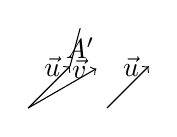
\begin{tikzpicture}
		\draw[->] (0, 0) --+ (30:1) node [left] {$\vec{v}$};
		\draw[->] (1, 0) --+ (45:0.75) node [left] {$\vec{u}$};
		\draw[->] (0, 0) --+ (45:0.75) coordinate (A) node [left] {$\vec{u}$};
		\draw[] (A) --+ (75:0.5) node [below] {$A'$};
	\end{tikzpicture}
\end{wrapfigure}
	Le produit scalaire de $\vec{u}$ par $\vec{v}$ est le produit de la longueur $\vec{v}$ et de la longueur algébrique du projeté orthogonal de $\vec{u}$ sur $\vec{v}$

	A', projeté orthogonal de A sur la droite portée de $\vec{v}$, passant pr 0. $\vec{OA'}$ est le projeté orthogonal de $\vec{u}$ sur $\vec{v}$

	\[\begin{array}{rcl}
				\vec{OA} \cdot \vec{OB} &=& OB.\overline{OA'} \\
	&=& OB \cdot OA \cos(\vec{OB}, \vec{OA})\end{array}\]

\paragraph{Remarque}
Si $\vec{u} = \vec{0}$ ou $\vec{v} = \vec{0}$ ou les les droites portées par $\vec{u} et \vec{v}$ orthogonales, alors $\vec{u}\cdot\vec{v} = 0$

\subsection{Définition analytique}
	On se donne un repère orthonormé. Dans ce repère, on se donne 2 vecteurs : $\vec{u} \begin{pmatrix}
		u_1 \\
		u_1
	\end{pmatrix}$ et $\vec{v} = \begin{pmatrix}
		v_1 \\
	v_2\end{pmatrix}$

	\[\vec{u}\cdot\vec{v} = u_1v_1 + u_2v_2\]

	\paragraph{Démonstration} On fixe A et B tels que $\vec{OA} = \vec{u}$ et $\vec{OB} = \vec{v}$

	$A = (u_1, u_2) $ et $B = (v_1, v_2)$ (coordonnées cartésiennes)

	$A$ et $B$ sont d'affixe respective 
	\[\begin{array}{rcccccl}
			A&=&u_1+iu_2 &et& B&=&v_1 + iv_2 \\
	A&=& r_Ae^{i\theta_A} && B &=& r_B e^{i\theta_B}\end{array}\]

	Maintenant :
	\[\begin{array}{rcl}
		\vec{OA}\cdot\vec{OB} &=& OA \cdot OB \cos (\theta) \\
						  &=& r_Ar_B \cos(\theta_B-\theta_A)\\
						  &=& r_Ar_B (\cos(\theta_B) \cos(\theta_A) + \sin(\theta_B) \sin(\theta_A) 
							&=& (r_A \cos(\theta_B)) (r_B \cos(\theta_B)) + (r_A \cos(\theta_A))(r_B\cos(\theta_A)) \\
							&=& u_1v_1 + u_2v_2\]

			\paragraph{Remarque} Le produit scalaire est symétrique : $\vec{u}\cdot\vec{v} = \vec{v}\cdot\vec{u}$

			\paragraph{Exemple} $D$ d'équation $ax + by +c=0$ passant par $P=(1, 4)$ et perpendiculaire  à $\Delta$ d'équation $-x+2y+1=0$

			$\Delta$ a pour vecteur directeur $\vec{u} = \begin{pmatrix}
				-2 \\
			-1\end{pmatrix}$ et $D \vec{v}=\begin{pmatrix}
				v_1 \\
				v_1
			\end{pmatrix}$

			On cherche $\vec{v}$ vecteur directeur de $D$ tel que $\vec{u}\cdot \vec{v} = 0$

			\[-2v_1 - v_2 = 0\], par exemple, $\vec{v} = \begin{pmatrix}
				-1\\
			-2\end{pmatrix}$ convient.

			$u_1 = -v_2$ et $u_2 = v_1$

			L'équation de $D$ est du type \[-2x -y +c = 0\] en utilisant P, on trouve $c=+$

			\paragraph{Remarque} $D \perp \{(x, y) | ax + by + c = 0\}$

			$D=\{(x, y) | bx - ay + c' = 0\}
